%%%%%%%%%%%%%%%%%%%%%%%%%%%%%%%%%%%%%%%%%%%%%%%%%%%%%%%%%%%%%%%%%%%%%%%%
% ICASSP 2027 -- reviewer-optimized working manuscript
% Technical content: pages 1--4. Page 5: references only.
%%%%%%%%%%%%%%%%%%%%%%%%%%%%%%%%%%%%%%%%%%%%%%%%%%%%%%%%%%%%%%%%%%%%%%%%

\documentclass{article}
\usepackage{spconf}
\usepackage{amsmath,amssymb,amsfonts,booktabs,graphicx}
\usepackage{array}
\usepackage{url}

\renewcommand{\dbltopfraction}{0.95}
\renewcommand{\dblfloatpagefraction}{0.90}
\renewcommand{\topfraction}{0.95}
\renewcommand{\floatpagefraction}{0.90}
\renewcommand{\textfraction}{0.04}

\newcommand{\NLL}{\mathrm{NLL}}
\newcommand{\KL}{D_{\mathrm{KL}}}
\newcommand{\argmin}{\operatorname*{arg\,min}}
\setlength{\textfloatsep}{7pt plus 1pt minus 2pt}
\setlength{\dbltextfloatsep}{7pt plus 1pt minus 2pt}
\setlength{\floatsep}{6pt plus 1pt minus 2pt}
\title{Cross-Layer Replacement Sharing for Model Compression}

\ifdefined\ANONYMOUS
  \name{Anonymous ICASSP 2027 submission}
  \address{}
\else
  \name{Yen-Han Lin \qquad Jen-Tzung Chien}
  \address{Institute of Electrical and Computer Engineering,\\
  National Yang Ming Chiao Tung University, Hsinchu, Taiwan}
\fi
\begin{document}
\ninept
\maketitle

\begin{abstract}
Cross-layer sharing provides an avenue to reduce large language model storage by reusing feed-forward weights across decoder depths, but effective sharing depends on which pretrained functions remain compatible when reused at different layers. We measure this compatibility through the directed full-model replacement cost and formulate the sharing under a fixed storage budget. A group replacement bound provides a practical criterion for grouping, while the final representative is selected in the actual donor-to-target direction. Across Llama-3.2-3B and Llama-3.1-8B, our method reaches 84.09\% and 85.92\% seven-task macro accuracy at the strongest structural operating points, compared with 65.06\% and 69.96\% for the strongest baseline. The advantage also persists after post-training quantization: the 25\% 8B INT8 model occupies 6.50~GiB while remaining within 0.51 percentage points of the dense teacher. Structural analyses further explain the role of directionality and the gap between pairwise replacement and joint deployment.
\end{abstract}
\begin{keywords}
large language model compression, cross-layer sharing, functional replacement, functional preservation, knowledge distillation
\end{keywords}

% ============================================================================
\section{Introduction}
% ============================================================================
Transformer decoders usually store an independent feed-forward network (FFN)
at every layer. Cross-layer sharing reduces this redundancy by reusing a
smaller set of FFN weights while retaining the original logical depth
\cite{dehghani2019universal,lan2020albert}. Related compression methods share
low-rank bases or approximate weight matrices through factorization
\cite{wang2025basis,wang2025svdllm}. Their effectiveness depends not only on
how many parameters are removed, but also on whether the resulting
parameterization can recover task capability.

Weight distance and activation similarity provide only indirect evidence for
cross-depth reuse. Two FFNs may appear locally similar yet cause different
end-to-end changes when exchanged, and the effect can reverse with the
replacement direction. We therefore score donor-to-target replacements inside
the frozen pretrained model and use the resulting replacement cost to
construct sharing groups.

Our method separates structural compression from subsequent recovery.
We first select sharing groups and their representatives using only the frozen
pretrained model, and then keep this structure fixed during all downstream
training. This allows us to evaluate three distinct stages: the model
immediately after compression, its ability to recover from ground-truth
supervision, and its ability to recover with additional teacher information.
We further test whether the recovered models remain effective after INT8 and
INT4 post-training weight quantization.

Our contributions are threefold. First, we introduce a directed full-model
replacement criterion that measures whether a pretrained FFN can serve another
decoder depth. Second, we formulate sharing under a fixed storage budget and
derive a group replacement bound that leads naturally to complete-link grouping
and directional representative selection. Third, we evaluate the resulting
structures across two Llama backbones and three compression levels, including
label-only recovery, teacher-assisted recovery, low-bit quantized deployment,
and structural analyses that connect the measured replacement quantities to
the final shared model.

% ============================================================================
\section{Related Work}
% ============================================================================

\textbf{Cross-layer parameter sharing.}
Parameter sharing reduces model size by reusing weights across network depth.
Universal Transformers apply recurrent parameter reuse, while ALBERT shares
parameters across encoder layers \cite{dehghani2019universal,lan2020albert}.
More recently, Basis Sharing represents multiple LLM layers using shared
low-rank bases with layer-specific coefficients \cite{wang2025basis}.
These methods exploit redundancy across depth, but do not directly determine
which pretrained functions can reliably serve other decoder depths. Our method
addresses this assignment problem using directed full-model replacement cost
rather than weight- or activation-level similarity.

\textbf{Low-rank model compression.}
Low-rank factorization reduces storage by approximating weight matrices with
smaller factors. SVD-LLM improves this process through truncation-aware data
whitening and post-truncation parameter updates \cite{wang2025svdllm}.
Unlike such layer-wise matrix factorization, our method reduces storage by
sharing pretrained functions across decoder depths.

\textbf{Post-compression recovery.}
Compressed models can recover task performance through supervised fine-tuning
or knowledge distillation, where a teacher transfers information through its
predictive distribution \cite{hinton2015distilling}. In our study, recovery is
kept separate from structural selection and is used only to evaluate the
recoverability of the frozen compression structure.

\textbf{Post-training quantization.}
Post-training quantization further reduces model storage after structural
compression. GPTQ uses approximate second-order information for weight
quantization, while AWQ uses activation statistics to protect salient weights
\cite{frantar2023gptq,lin2024awq}. We instead use a common training-free
quantization procedure to test whether the structural advantage persists under
INT8 and INT4 deployment.

\begin{figure*}[t]
\centering
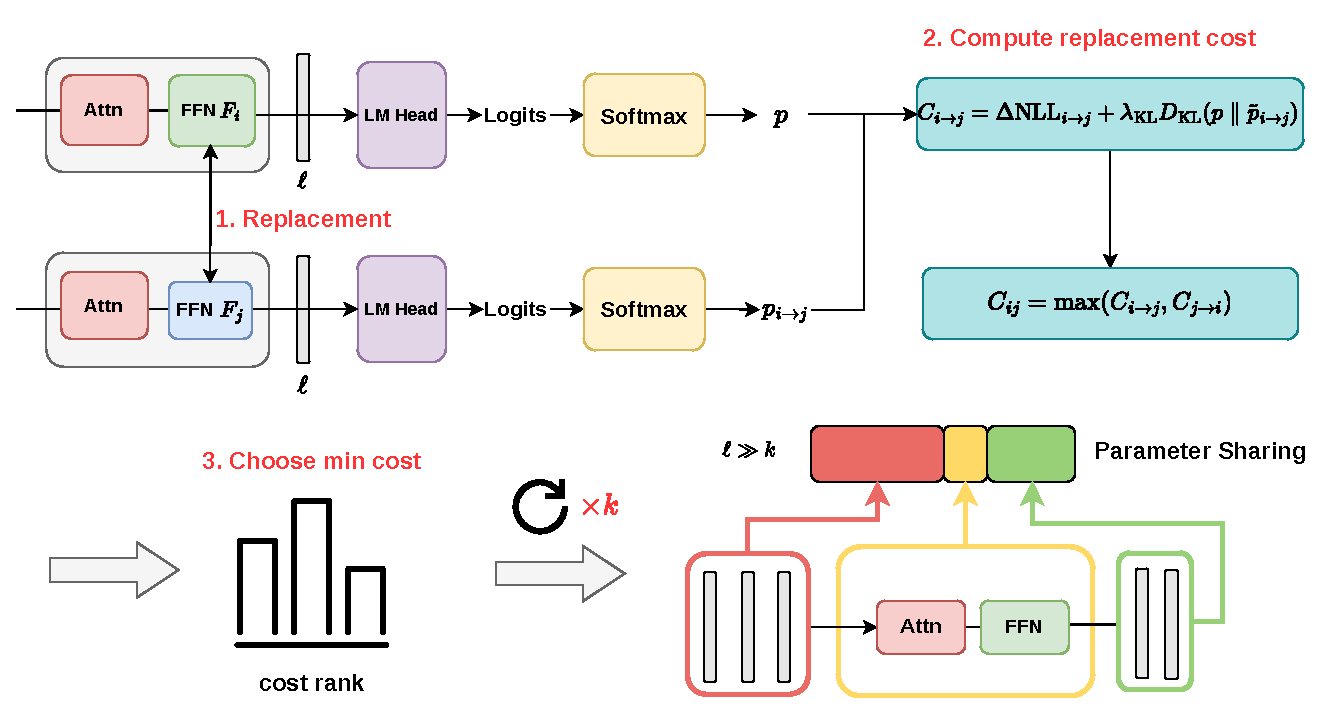
\includegraphics[width=0.82\textwidth]{Figure/replace.pdf}
\caption{\textbf{Framework and evaluation logic.} Directed full-model
replacements determine cross-depth compatibility, complete-link forms a fixed
number of groups, and the selected representative initializes each shared FFN.
The structure is then frozen and evaluated under Pure, CE, and CE+KD recovery.}
\label{fig:framework}
\end{figure*}

% ============================================================================
\section{Budgeted Functional Preservation}
% ============================================================================

\subsection{Directed replacement cost}

Let $M_0$ contain frozen decoder FFNs $F_1,\ldots,F_L$. For donor $i$ and
target $j\neq i$, we replace $F_j$ by $F_i$ while keeping the remaining model
fixed. Let $p_0$ and $p_{i\to j}$ denote the reference and intervened
next-token distributions. We define
\begin{equation}
C_{i\to j}
=
\underbrace{\NLL(p_{i\to j})-\NLL(p_0)}_{\Delta\NLL_{i\to j}}
+
\lambda_{\mathrm{KL}}
\mathbb E\!\left[
\KL\!\left(p_0\middle\|p_{i\to j}\right)
\right].
\label{eq:directed-cost}
\end{equation}
The NLL term measures the observed-token change, while the KL term captures
redistribution over the full predictive distribution, with
$\lambda_{\mathrm{KL}}=1$. In general,
$C_{i\to j}\neq C_{j\to i}$.

\subsection{Budgeted replacement objective}

A budget of $K<L$ stored FFNs partitions the $L$ layers into $K$ sharing
groups. For a sharing group $\mathcal G$ and candidate representative
$m\in\mathcal G$, define
\begin{align}
d(m;\mathcal G)
&=
\max_{j\in\mathcal G\setminus\{m\}} C_{m\to j},
\qquad d(m;\{m\})=0, \nonumber\\[-0.5mm]
\delta(\mathcal G)
&=
\min_{m\in\mathcal G} d(m;\mathcal G).
\label{eq:group-donor}
\end{align}
Thus, $\delta(\mathcal G)$ is the best representative cost: the smallest
worst-case replacement cost achievable by selecting one group member.
Let $\mathcal P$ denote a partition of the layer indices
$\{1,\ldots,L\}$. The ideal fixed-budget objective is
\begin{equation}
\mathcal D_K^\star
=
\min_{\mathcal P:\,|\mathcal P|=K}
\max_{\mathcal G\in\mathcal P}
\delta(\mathcal G).
\label{eq:preservation-objective}
\end{equation}
Thus, $K$ fixes the number of stored FFNs, while $\mathcal D_K^\star$ is the
minimum achievable worst-group cost under that budget.

\subsection{Greedy replacement grouping}

Joint optimization over partitions and representatives is combinatorial.
We therefore define, for $i\neq j$, the mutual replacement cost and its
corresponding group bound as
\begin{equation}
\bar C_{ij}
=
\max\{C_{i\to j},C_{j\to i}\},
\qquad
\Delta(\mathcal G)
=
\max_{\substack{i,j\in\mathcal G\\ i\neq j}}
\bar C_{ij},
\quad
\Delta(\{i\})=0.
\label{eq:group-bound}
\end{equation}
Here, $\bar C_{ij}$ keeps the more costly replacement direction, while
$\Delta(\mathcal G)$ is the largest mutual replacement cost within the group.
For any representative $m\in\mathcal G$ and
$j\in\mathcal G\setminus\{m\}$,
$C_{m\to j}\leq\bar C_{mj}\leq\Delta(\mathcal G)$; hence
\begin{equation}
\delta(\mathcal G)\leq\Delta(\mathcal G).
\label{eq:group-bound-relation}
\end{equation}
Thus, $\Delta(\mathcal G)$ provides a conservative group replacement bound,
while the final representative is selected using the directed replacement cost.

For two current groups, define
\begin{equation}
D_{\mathrm{CL}}(A,B)
=
\max_{i\in A,\,j\in B}\bar C_{ij}.
\label{eq:complete-link}
\end{equation}
The bound of the merged group satisfies
\begin{equation}
\Delta(A\cup B)
=
\max\{\Delta(A),\Delta(B),D_{\mathrm{CL}}(A,B)\}.
\label{eq:merge-identity}
\end{equation}
At greedy step $t$, let $\mathcal P_t$ denote the current partition and $M_t=\max_{\mathcal G\in\mathcal P_t}\Delta(\mathcal G)$ its maximum group bound. After merging $A$ and $B$, the new maximum is $\max\{M_t,D_{\mathrm{CL}}(A,B)\}$. Thus, choosing the candidate pair with
minimum $D_{\mathrm{CL}}$ gives a one-step minimax complete-link rule without
claiming global optimality.

After $K$ groups remain, denote them by
$\mathcal G_1,\ldots,\mathcal G_K$. We then select each representative by
\begin{equation}
m_k^\star
=
\argmin_{m\in\mathcal G_k}
\max_{j\in\mathcal G_k\setminus\{m\}}
C_{m\to j}.
\label{eq:representative}
\end{equation}
Consequently,
\begin{equation}
\delta_{\max}
\equiv
\max_k \delta(\mathcal G_k)
\leq
\max_k \Delta(\mathcal G_k)
\equiv
\Delta_{\max}.
\label{eq:deployment-bound}
\end{equation}

In implementation, each logical layer $\ell\in\mathcal G_k$ uses the FFN
shared by group $\mathcal G_k$ together with a layer-specific parallel
low-rank adapter, following the low-rank residual parameterization of
\cite{hu2022lora}. The effective FFN is
\begin{equation}
\widetilde F_\ell(x)
=
F_{\mathrm{shared}}^{(k)}(x)
+
A_\ell(x),
\label{eq:parallel-adapter}
\end{equation}
where $x\in\mathbb R^D$ is the FFN input,
$F_{\mathrm{shared}}^{(k)}$ is initialized from $F_{m_k^\star}$, and $A_\ell(x)=U_\ell V_\ell x$, with
$V_\ell\in\mathbb R^{\rho\times D}$,
$U_\ell\in\mathbb R^{D\times\rho}$, and $\rho=64$.
The shared FFN and adapter operate in parallel on the same layer input.
All adapter parameters are included in the reported model size, and the
sharing groups and representatives are fixed before recovery.
Equation~\eqref{eq:deployment-bound} characterizes isolated replacements;
simultaneous sharing may introduce additional interactions, which we evaluate
separately. To compare the simultaneous model with the single-replacement
scale, let $p_{\mathrm{shared}}$ be the predictive distribution after deploying
the complete sharing partition and define the per-layer joint cost
\begin{equation}
C^\star
=
\frac{1}{L}\left[
\NLL(p_{\mathrm{shared}})-\NLL(p_0)
+\lambda_{\mathrm{KL}}\mathbb E\!\left[
\KL\!\left(p_0\middle\|p_{\mathrm{shared}}\right)
\right]\right].
\label{eq:c-star}
\end{equation}
We use $L=28$ for Llama-3.2-3B and $L=32$ for Llama-3.1-8B.
% ============================================================================
\section{Experiments}
\label{sec:experiments}
%

\begin{table*}[t]
\centering
\caption{\textbf{Seven-task macro accuracy (\%).}
Pure evaluates the frozen compressed checkpoint without training.
CE and CE+KD report mean$\pm$SD over paired seeds $\{42,43,44\}$.
Bold denotes the best CE or CE+KD result at each operating point.}
\label{tab:main}

\vspace{1.8mm}

\setlength{\tabcolsep}{2.15pt}
\renewcommand{\arraystretch}{1.02}

\begin{minipage}[t]{0.485\textwidth}
\centering
\textbf{(a) Llama-3.2-3B}\\[0.4mm]
{\footnotesize Dense refs.: 36.93 pretrained / 82.30 task-trained}\\[0.7mm]

\begin{tabular}{@{}c l r r r@{}}
\toprule
Target & Method & Pure & CE & CE+KD \\
\midrule
15\%
& Basis Sharing & 33.20 & 71.04$\pm$0.12 & 71.28$\pm$0.52 \\
& SVD-LLM       & 33.20 & 57.36$\pm$20.32 & 70.78$\pm$0.13 \\
& Ours          & 33.21 & \textbf{85.35$\pm$0.17}
                         & \textbf{84.83$\pm$0.47} \\

\addlinespace[1.2pt]

20\%
& Basis Sharing & 33.20 & 48.91$\pm$13.84 & 68.15$\pm$0.54 \\
& SVD-LLM       & 33.20 & 33.49$\pm$0.22 & 67.32$\pm$0.28 \\
& Ours          & 33.95 & \textbf{85.07$\pm$0.54}
                         & \textbf{85.06$\pm$0.08} \\

\addlinespace[1.2pt]

25\%
& Basis Sharing & 33.22 & 33.73$\pm$0.48 & 65.06$\pm$0.20 \\
& SVD-LLM       & 33.22 & 33.62$\pm$0.37 & 63.58$\pm$0.73 \\
& Ours          & 33.77 & \textbf{84.60$\pm$0.12}
                         & \textbf{84.09$\pm$0.18} \\
\bottomrule
\end{tabular}
\end{minipage}
%
\hfill
%
\begin{minipage}[t]{0.485\textwidth}
\centering
\textbf{(b) Llama-3.1-8B}\\[0.4mm]
{\footnotesize Dense refs.: 46.71 pretrained / 86.85 task-trained}\\[0.7mm]

\begin{tabular}{@{}c l r r r@{}}
\toprule
Target & Method & Pure & CE & CE+KD \\
\midrule
15\%
& Basis Sharing & 33.27 & 76.05$\pm$0.39 & 76.43$\pm$0.47 \\
& SVD-LLM       & 33.21 & 74.43$\pm$0.19 & 75.31$\pm$0.89 \\
& Ours          & 36.27 & \textbf{85.54$\pm$0.33}
                         & \textbf{86.14$\pm$0.33} \\

\addlinespace[1.2pt]

20\%
& Basis Sharing & 33.20 & \textbf{72.81$\pm$0.75} & 73.89$\pm$0.54 \\
& SVD-LLM       & 33.20 & 58.77$\pm$21.74 & 73.01$\pm$0.74 \\
& Ours          & 33.65 & 68.04$\pm$17.02
                         & \textbf{85.94$\pm$0.34} \\

\addlinespace[1.2pt]

25\%
& Basis Sharing & 33.20 & 33.16$\pm$0.04 & 69.96$\pm$0.64 \\
& SVD-LLM       & 33.21 & 33.32$\pm$0.26 & 69.64$\pm$0.34 \\
& Ours          & 34.05 & \textbf{81.67$\pm$5.96}
                         & \textbf{85.92$\pm$0.36} \\
\bottomrule
\end{tabular}
\end{minipage}

\vspace{-0.5mm}
\end{table*}
\subsection{Setup and evaluation}

We evaluate Llama-3.2-3B and Llama-3.1-8B
\cite{grattafiori2024llama3} at nominal compression targets of
15\%, 20\%, and 25\%. We compare our method with Basis Sharing
\cite{wang2025basis} and SVD-LLM \cite{wang2025svdllm}. Since the three
methods represent compressed weights differently, the nominal targets are used
to identify comparable operating points. Actual parameter reduction and
serialized model size are measured separately.

Evaluation uses multiple-choice log-probability scoring on PIQA, Social IQa,
WinoGrande, ARC-Challenge, ARC-Easy, HellaSwag, and OpenBookQA
\cite{bisk2020piqa,sap2019socialiqa,sakaguchi2021winogrande,clark2018arc,
zellers2019hellaswag,mihaylov2018openbookqa}. We report the unweighted
seven-task macro accuracy.

To separate structural compression from recovery, each frozen compressed
checkpoint is evaluated under three settings. \textbf{Pure} uses no additional
training, \textbf{CE} uses ground-truth supervision only, and \textbf{CE+KD}
adds a frozen task-trained teacher for the corresponding backbone:
\begin{equation}
\mathcal L_{\mathrm{CE+KD}}
=
\mathcal L_{\mathrm{CE}}
+
\lambda_{\mathrm{KD}}\tau^2
\KL\!\left(p_T^{(\tau)}\middle\|p_S^{(\tau)}\right),
\label{eq:kd}
\end{equation}
where $p_T^{(\tau)}$ and $p_S^{(\tau)}$ are the teacher and student predictive
distributions at temperature $\tau$. CE and CE+KD use paired student seeds
$\{42,43,44\}$. Training data, optimization budget, checkpoint selection,
teacher, and evaluator are fixed across methods, and recovery never changes
the compression structure selected beforehand.

\medskip
\noindent\textbf{Recovery protocol.}
Recovery uses 156,668/161,781 examples and 7,500/10,000 updates for 3B/8B,
with maximum sequence length 384 and effective batch sizes 32/8. We use AdamW
($\beta_1=0.9$, $\beta_2=0.999$, weight decay $0.01$). Peak learning rates
for the main model, shared FFNs, and layer-specific adapters are
$(3,5,8)\times10^{-5}$ for 3B and $(2.5,4,6)\times10^{-5}$ for 8B, with
warmup--cosine scheduling and gradient clipping at $1.0$.

CE remains teacher-free, while CE+KD uses the same frozen teacher across
methods and compression levels, with $\tau=2$ and
$\lambda_{\mathrm{KD}}=1$. We validate every 500 updates on at most 2,048
held-out examples and retain the checkpoint with the lowest held-out decision
CE; step 0 and final test sets are never used for checkpoint selection.





% ============================================================================
\subsection{Recovery under increasing compression}
% ============================================================================

Table~\ref{tab:main} first shows that the compressed checkpoint alone is not a
good measure of the final task model. Pure accuracy remains low for all three
methods, although our method is slightly higher at several operating points.
The main difference appears after recovery.

With CE+KD, our method achieves the highest macro accuracy at all six
backbone--compression settings. At 15/20/25\% compression, the advantage over
the strongest baseline is 13.55/16.91/19.03 percentage points on 3B and
9.71/12.05/15.96 points on 8B. The gap becomes larger as compression becomes
stronger.

From 15\% to 25\%, our CE+KD accuracy decreases by only 0.74 points on 3B and
0.22 points on 8B. In contrast, Basis Sharing decreases by 6.22/6.47 points
and SVD-LLM by 7.20/5.67 points. Thus, the structure selected by our method
remains much easier to recover as the storage budget becomes tighter.


\begin{figure*}[!t]
\centering
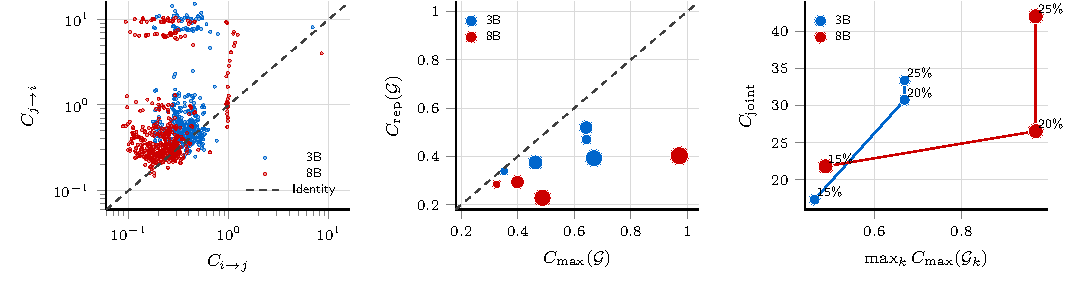
\includegraphics[width=0.94\textwidth]
{Figure/structural_validation.pdf}
\caption{Structural validation.
(a) Directed replacement costs exhibit clear source--target asymmetry.
(b) The best representation cost satisfies
$C_{\mathrm{rep}}(\mathcal G)\leq C_{\max}(\mathcal G)$ for every observed group.
(c) Per-layer joint cost $C^\star$ is compared directly with
$\max_k C_{\max}(\mathcal G_k)$; the dashed line marks equality.}
\label{fig:structural}
\vspace{-1mm}
\end{figure*}


CE-only recovery provides a second observation. On 3B, our method remains
stable across all three compression levels. On 8B, CE becomes seed-sensitive
at the harder operating points: the seed standard deviation decreases from
17.02 to 0.34 points at 20\% and from 5.96 to 0.36 points at 25\% when CE+KD
is used. KD therefore mainly stabilizes difficult recovery settings rather
than uniformly increasing the mean accuracy.

At 25\% compression, our method also achieves the highest accuracy on all seven
benchmarks for both backbones. Across 36 paired seed-level comparisons against
Basis Sharing and SVD-LLM, all task-stratified bootstrap intervals remain
above zero.



\subsection{Structural validation}

We next examine whether the structural measurements used by our method support
the design choices in Sec.~3.

\noindent\textbf{Directional replacement.}
Figure~\ref{fig:structural}(a) shows clear donor--target asymmetry. The median
$|C_{i\to j}-C_{j\to i}|$ is 0.221 on 3B and 0.140 on 8B, while the 90th
percentiles reach 7.31 and 6.24. This supports the directed cost
$C_{i\to j}$ rather than a symmetric similarity.

\noindent\textbf{Group replacement bound.}
Figure~\ref{fig:structural}(b) compares the group replacement bound
$\Delta(\mathcal G)$ with the best representative cost $\delta(\mathcal G)$.
Every observed group satisfies $\delta(\mathcal G)\leq\Delta(\mathcal G)$,
as required by Eq.~\eqref{eq:group-bound-relation}, with a maximum gap of
0.569. The gap measures how conservative the group bound is relative to the
selected representative.

\noindent\textbf{Pairwise versus joint deployment.}
Figure~\ref{fig:structural}(c) compares the worst selected group cost with the
per-layer simultaneous cost in Eq.~\eqref{eq:c-star}. As compression increases,
$C^\star$ rises from 0.619 to 1.193 on 3B and from 0.682 to 1.314 on 8B. The
20\% and 25\% structures can share the same $\Delta_{\max}$ while producing
different $C^\star$. All six observations lie above the dashed equality line,
so pairwise quantities guide structural selection but do not numerically bound
the simultaneous per-layer cost.

\noindent\textbf{Ablation.}
At the 3B--20\% operating point, the full method reaches 85.11\% CE+KD accuracy
with $C^\star=1.099$. Removing directionality lowers accuracy to
83.29\% and raises $C^\star$ to 1.216. A symmetric donor has higher
Pure accuracy (34.75\%) but raises $C^\star$ to 3.132 and lowers
CE+KD to 80.06\%, showing that immediate Pure quality does not determine
recoverability. Two-way mean and single-link yield the same frozen structure
at this operating point and therefore are not independent comparisons.

\noindent\textbf{Accounting and scope.}
Basis Sharing and SVD-LLM closely match the nominal 15/20/25\% standalone
reductions, while ours realizes 13.95/\allowbreak20.93/\allowbreak25.58\% on 3B and
15.26/\allowbreak19.63/\allowbreak26.17\% on 8B, including all stored parameters. Logical depth and
FFN execution count are unchanged, so we claim storage rather than inherent
FLOP reduction.


% ============================================================================
\subsection{Quantized deployment}
\label{sec:quantized}
% ============================================================================

Finally, we test whether the structural advantage persists under low-precision
deployment. We quantize the recovered Llama-3.1-8B models at the 15\% and
25\% structural operating points while keeping the sharing structure fixed.

\begin{figure}[!t]
\centering
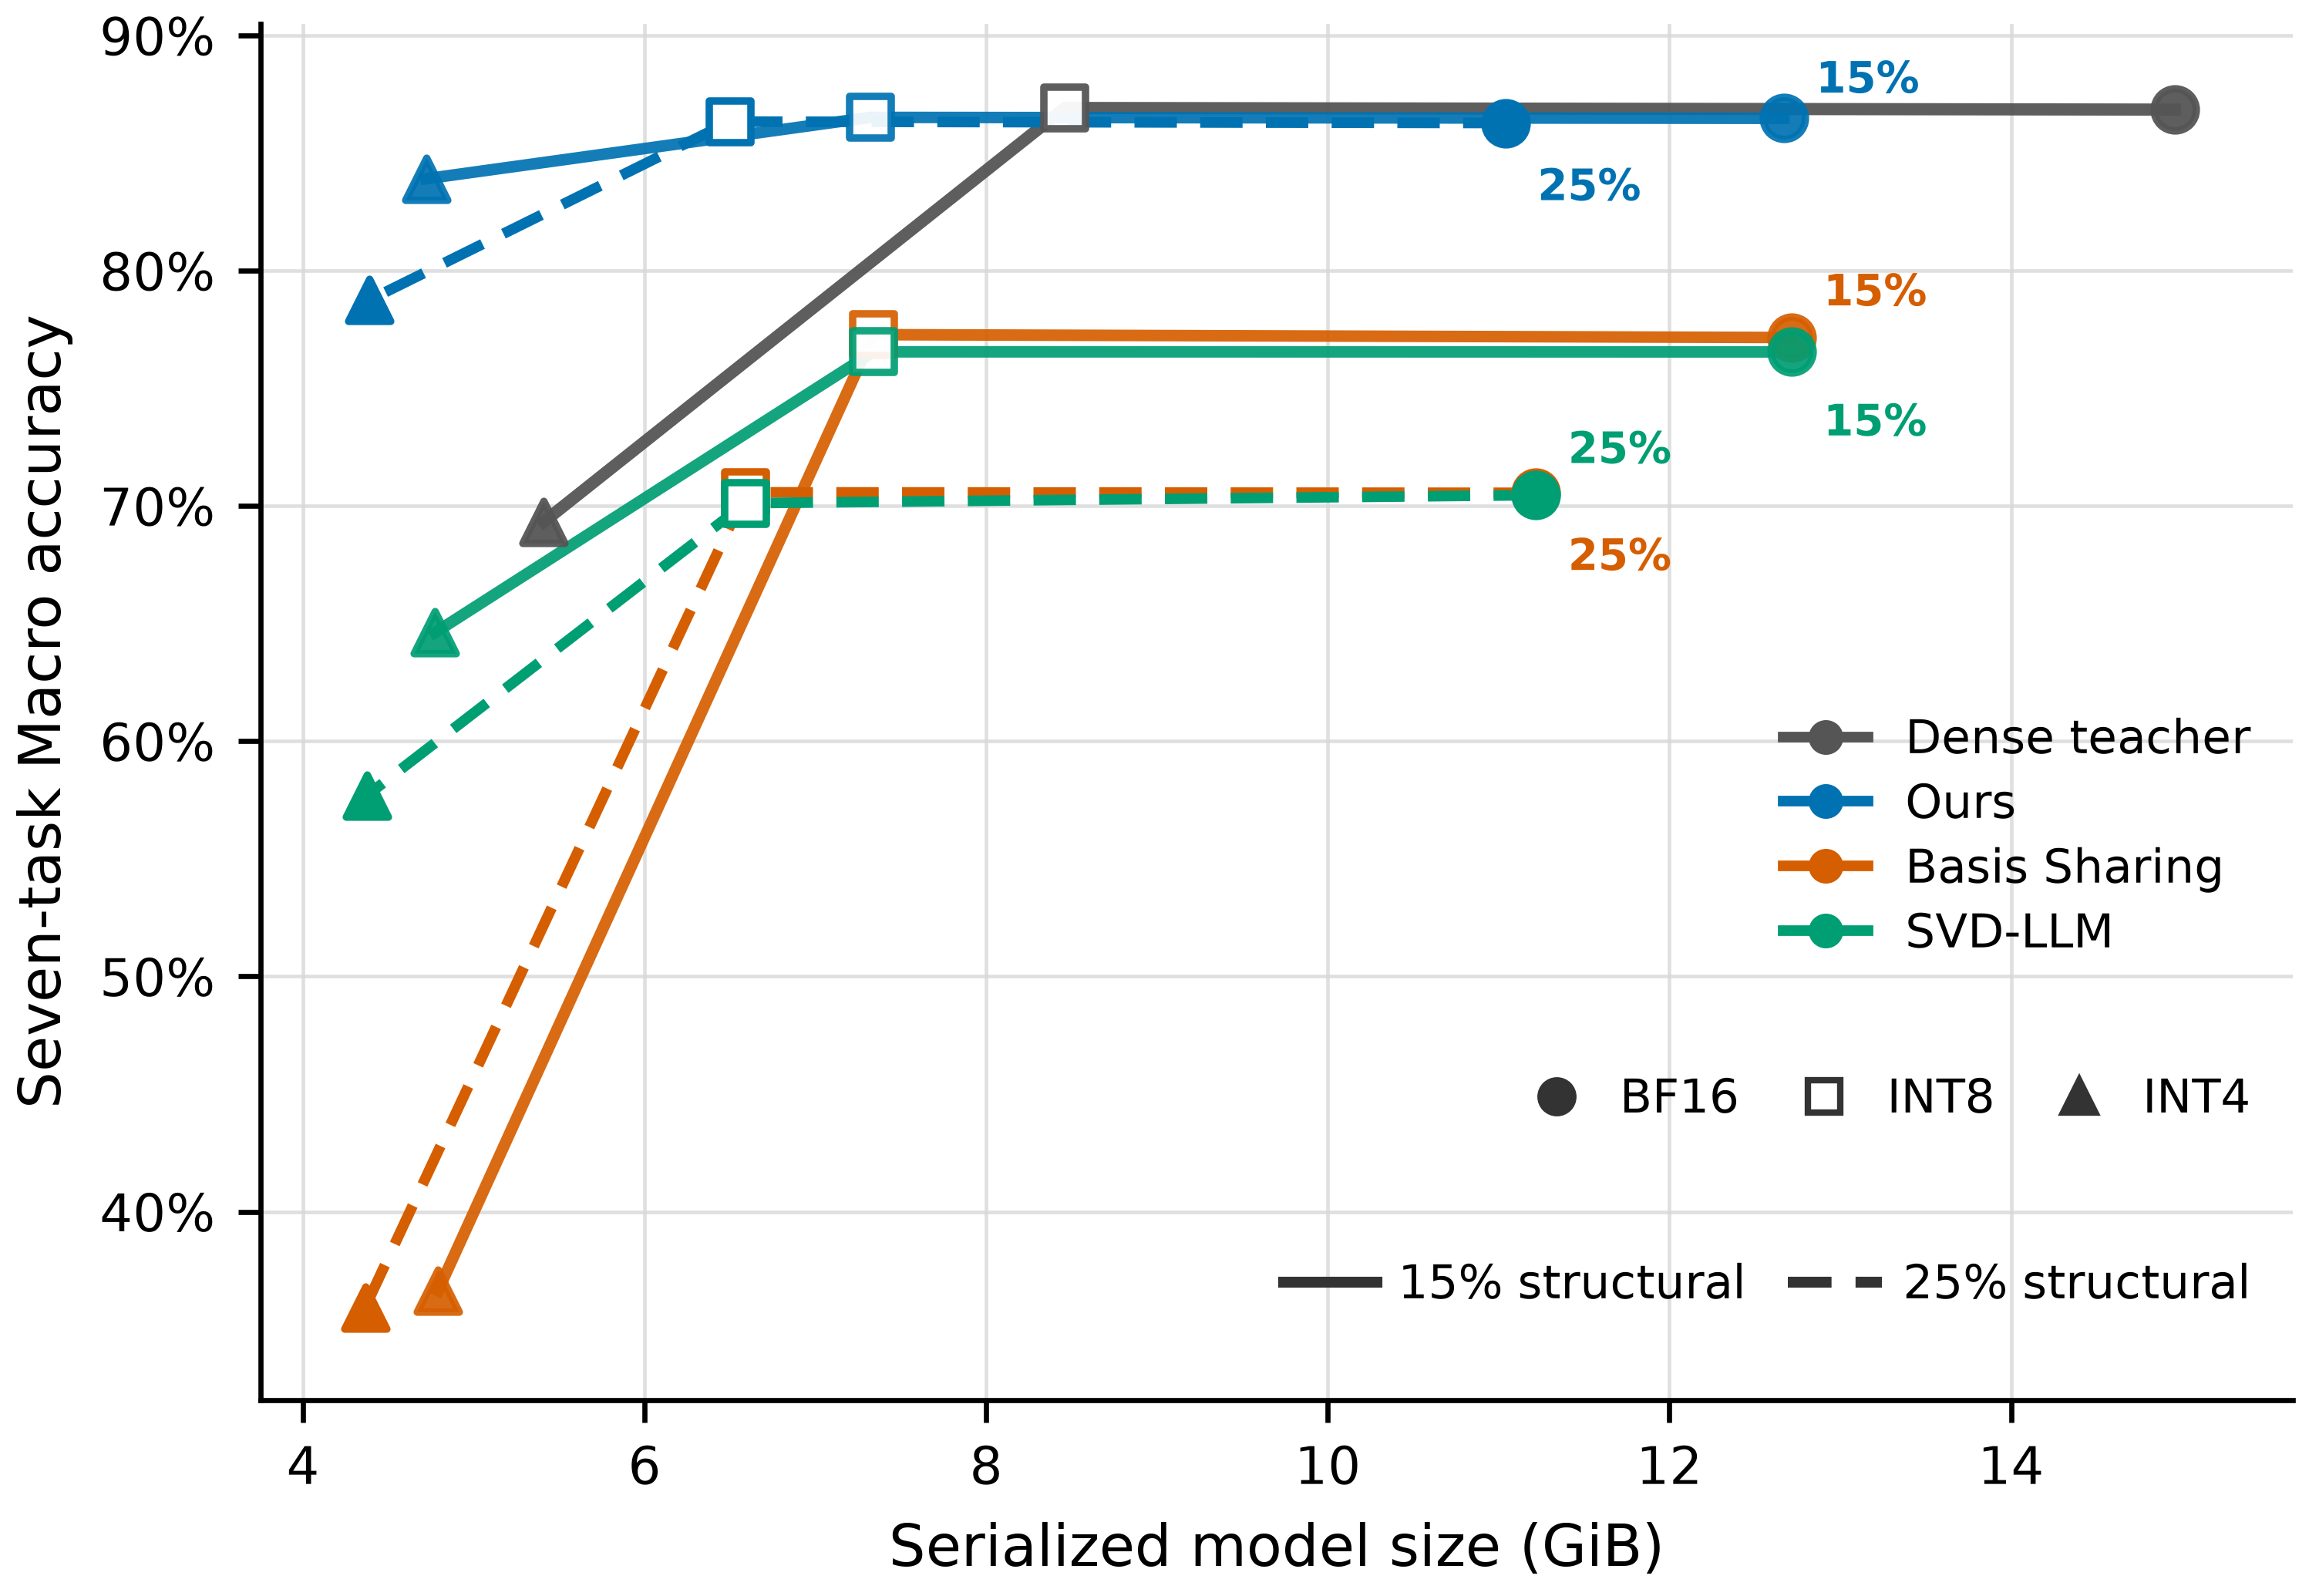
\includegraphics[width=0.88\columnwidth]
{Figure/fig_quantization_15_25_storage_accuracy.png}
\caption{\textbf{Quantized Llama-3.1-8B storage--accuracy trade-off.}
BF16, INT8, and INT4 are shown at 15\% and 25\% structural compression;
upper-left points are preferable.}
\label{fig:quantization}
\vspace{-1mm}
\end{figure}

\noindent\textbf{Quantization protocol.}
We use training-free weight-only round-to-nearest quantization: INT8 is
symmetric per output channel, INT4 is group-128, and activations remain BF16.
The same layer policy and evaluator are used for all methods; shared FFNs and
private adapters are both eligible. Packed weights are dequantized for BF16
compute, so we make no integer-kernel speed claim. No calibration, QAT, or
post-quantization recovery is used.

For ours, INT8 reaches 86.52\% at 7.32~GiB for 15\% structural compression and
86.34\% at 6.50~GiB for 25\%, reducing dense-BF16 storage by 51.07\% and
56.53\% while remaining 0.33 and 0.51 points below the teacher. The latter
saves another 0.82~GiB over 15\% INT8 for 0.18 points; small BF16--INT8
differences are not interpreted as gains.

Under INT4, ours loses 2.57/7.52 points at 15/25\%, versus 40.51/34.63 for
Basis Sharing and 11.93/12.77 for SVD-LLM. At 15\%, ours still reaches 83.91\%,
compared with 36.65\% and 64.62\%, respectively.

\noindent\textbf{Conclusion.}
Directed replacement yields recoverable sharing; 25\% INT8 retains 86.34\% at
6.50~GiB and stays robust.

% ============================================================================
% Page 5: references
% ============================================================================
\clearpage

\bibliographystyle{IEEEbib}
\bibliography{references}

\end{document}
